\chapter{Kontekstfrie Sprog}

I det tidligere kapitel om endelige automater, så vi den klasse af sprog som de genkender, regulære sprog, men vi så også eksempler på sprog som ikke er regulære, og hvordan dette kan bevises. I dette kapitel vil vi introducere \textit{kontekstfrie grammatikker} som er stærkere end endelige automater i deres deskriptionskraft. Sprogene der genkendes af kontekstfrie grammatikker kaldes \textit{kontekstfrie sprog}. Ydermere introducerer vi \textit{stakautomater} (pushdown automata på engelsk) som er en klasse af maskiner der genkender kontekstfrie sprog.

\section{Kontekstfrie Grammatikker}
En grammatik består af en samling af \textbf{substitueringsregler}, også kaldet \textit{produktioenr}. Hver regel forekommer som en linje i grammatikken,  og består af et symbol efterfulgt af en pil efterfulgt af en streng. Følgende grammatik er et eksempel på en kontekstfri grammatik $G_{1}$:
\begin{equation}
  \tag{$G_{1}$}
  \begin{split}
  A &\rightarrow \mathtt{0}A \mathtt{1}\\
  A &\rightarrow B\\
  B &\rightarrow \mathtt{\#}
\end{split}
  \label{eqn:G1}
\end{equation}

Symbolet på venstresiden kaldes en \textit{variabel}\footnote{Kært barn har mange navne, jeg har også hørt non-terminal og, simpelt, LHS.}. Strengen (højresiden) består af variabler og andre symboler, kaldet \textit{terminale}. Terminale minder om alfabetet fra en endelig automat, da disse er de endelige symboler, der udgør en resulterende streng\footnote{Dette vil vi komme ind på i mere detalje senere.}. Variabler er oftest repræsenteret som store bogstaver, hvor terminale kan være små bogstaver, tal, eller specielle symboler (såsom \#.) En af variablerne (venstrehåndssiden) bliver udpeget til at være \textbf{startvariablen}. Denne variabel skal alle udledninger\footnote{En udledning bliver beskrevet i mere detalje i næste afsnit.} af grammatikken starte på (analogt til en start state i en endelig automat.)

For at beskrive et sprog med en grammatik, \textit{udleder} vi strenge fra grammatikken. Dette bliver gjort systematisk ved at \textit{substituere} variabler med andre variabler eller terminale. Eksempeltvis kan gramatikken \ref{eqn:G1} udlede strengen \texttt{000\#111}. En udledning af denne streng i \ref{eqn:G1} er følgende: $A \Rightarrow \mathtt{0}A \mathtt{1} \Rightarrow \mathtt{00}A \mathtt{11} \Rightarrow \mathtt{000}A \mathtt{111} \Rightarrow \mathtt{000}B \mathtt{111} \Rightarrow \mathtt{000\#111}$. En måde hvorpå du kan vise dette grafisk er \textit{parse-træer}. Et eksempel kan ses i Figur~\ref{fig:parsetreeg1}, som viser et parsetræ for strengen \texttt{000\#111} i grammatikken \ref{eqn:G1}.

\begin{figure}[ht]
  \centering
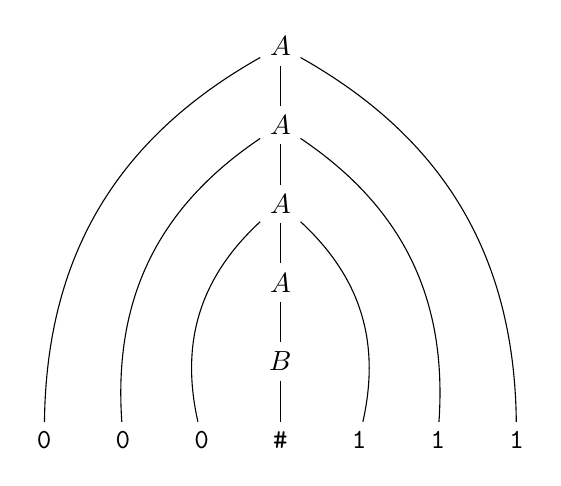
\begin{tikzpicture}[>=latex]
  % Nodes
  \node (0a) at (0,0) {\texttt{0}};
  \node (0b) at (1,0) {\texttt{0}};
  \node (0c) at (2,0) {\texttt{0}};
  \node (sharp) at (3,0) {\texttt{\#}};
  \node (1a) at (4,0) {\texttt{1}};
  \node (1b) at (5,0) {\texttt{1}};
  \node (1c) at (6,0) {\texttt{1}};

  % Upper nodes
  \node (B) at (3,1) {$B$};
  \node (A4) at (3,2) {$A$};
  \node (A3) at (3,3) {$A$};
  \node (A2) at (3,4) {$A$};
  \node (A1) at (3,5) {$A$};

  % Lines going down
  \draw[-] (B) to (sharp);
  \draw[-] (A4) to (B);
  \draw[-] (A3) to (A4);
  \draw[-] (A2) to (A3);
  \draw[-] (A1) to (A2);

  % Lines going to terminals
  \draw[-] (A1) to[bend right] (0a);
  \draw[-] (A1) to[bend left] (1c);
  \draw[-] (A2) to[bend right] (0b);
  \draw[-] (A2) to[bend left] (1b);
  \draw[-] (A3) to[bend right] (0c);
  \draw[-] (A3) to[bend left] (1a);

\end{tikzpicture}
  \caption{\label{fig:parsetreeg1} Parse-træ for \texttt{000\#111} i \ref{eqn:G1}}
\end{figure}


Alle strenge du kan udlede på denne måde er en del af sproget, og udgør tilsammen det kontekstfri sprog som \ref{eqn:G1} genkender. Hvis du ikke har lagt mærke til det nu, er denne meget simple kontekstfri grammatik faktisk et eksempel på et sprog der \textbf{ikke} kan genkendes af en endelig automat. Ofte, fremfor at skrive $A \rightarrow \mathtt{0}A \mathtt{1}$ og så på en ny linje skrive $A \rightarrow B$, så skriver man blot $A \rightarrow \mathtt{0} A \mathtt{1} | B$, hvor du kan se \texttt{|} som ``eller''.

Vi vil nu kigge på den formelle definition på en kontekstfri grammatik.

\begin{definition}[Formel Definition på en Kontekstfri Grammatik]
  En \textbf{kontekstfri grammatik}   er en 4-tuple $(V, \Sigma, R, S)$, hvor
  \begin{enumerate}
    \item $V$ er et endeligt sæt kaldet \textbf{variabler}
    \item $\Sigma$ er et endeligt sæt, disjunkt fra $V$, kaldet \textbf{terminaler}
    \item $R$ er et endeligt sæt af \textbf{regler}, hvor hver regel er en streng af variabler og terminaler og en variabel
    \item $S \in V$ er startvariablen.
  \end{enumerate}

\end{definition}

Givet $u, v$ og $w$ er strenge af variabler, og terminale, og $A \rightarrow w$ er en regel af grammatikken, så siger vi at $uAv$ giver (\textit{yields}) $uwv$, skrevet $uAv \Rightarrow uwv$. Vi siger at $u$ udleder $v$, skrevet, $u \stackrel{*}{\Rightarrow} v$, hvis $u = v$, eller hvis en sekvens $u_{1}, u_{2}, \ldots, u_{k}$ eksisterer når $k \geq 0$ og $u \Rightarrow u_{1} \Rightarrow u_{2} \Rightarrow \ldots \Rightarrow u_{k} \Rightarrow v$. Sproget af grammatikken er $\{w \in \Sigma* | S \stackrel{*}{\Rightarrow} w\}$.

\newpage
\section{Tvetydighed}%
\label{sec:tvetydighed}

En grammatik der kan generere den sammen streng på to eller flere forskellige måder (og dermed have mere end ét parsetræ for én streng), kaldes \textit{tvetydig}. For eksempel er den følgende grammatik tvetydig:
\[
\langle EXPR \rangle \rightarrow \langle EXPR \rangle + \langle EXPR \rangle | \langle EXPR \rangle + \langle EXPR \rangle | ( \langle EXPR \rangle ) | a
\]

Strengen $\mathtt{a + a \times a}$ kan generes tvetydigt: enten $$\langle EXPR \rangle \Rightarrow \langle EXPR \rangle + \langle EXPR \rangle \Rightarrow \langle EXPR \rangle + \langle EXPR \rangle \times \langle EXPR \rangle \Rightarrow \cdots \Rightarrow a + a \times a$$ eller $$\langle EXPR \rangle \Rightarrow \langle EXPR \rangle \times \langle EXPR \rangle \Rightarrow \langle EXPR \rangle + \langle EXPR \rangle \times \langle EXPR \rangle \Rightarrow \cdots \Rightarrow a + a \times a$$.

\begin{definition}[Tvetydighed]
En streng $w$ er udledt \textbf{\textit{tvetydigt}} i en kontekstfri grammatik $G$ hvis den har to eller flere venstremest udledninger. Grammatik $G$ er \textit{tvetydig} hvis den genererer en streng tvetydigt.
\end{definition}

Ofte, hvis man har en tvetydig grammatik, er det muligt at konvertere den til en grammatik der ikke er tvetydig. Dog er dette ikke muligt for alle sprog. Sprog hvor dette \textbf{ikke} gælder kalder vi \textbf{i sig selv tvetydige} (inherently ambiguous.)

\newpage
\section{Chomsky Normal Form}%
\label{sec:cnf}

Chomsky Normal Form er en simple form af en kontekstfri grammatik.

\begin{definition}[Chomsky Normal Form]
  En kontekstfri grammatik er i \textbf{\textit{Chomsky Normal Form}} hvis hver regel har formen
  \begin{equation*}
\begin{split}
  A &\rightarrow BC\\
  A &\rightarrow a
\end{split}
  \end{equation*}
  hvor $a$ er enhver terminal, og $A, B$ og $C$ er enhver variabel, dog må $B$ og $C$ ikke være startvariablen. Derudover tillader vi reglen $S \rightarrow \varepsilon$, hvor $S$ er startvariablen.
\end{definition}

\begin{theorem}
Ethvert kontekstfri sprog er genereret af en kontekstfri grammatik i Chomsky Normal Form.
\end{theorem}

Vi vil vise at vi kan konvertere enhver grammatik til chomsky normal form. Vi vil gøre dette ved at fjerne alle regler der går imod betingelserne for CNF, og erstatte med regler der overholder. Først tilføjer vi en ny startvariabel, og eliminerer alle regler af formen $A \rightarrow \varepsilon$ (kaldet $\varepsilon$-regler.) Vi eliminerer også alle \textbf{unit rules}, som har formen $A \rightarrow B$. Til sidst konverterer vi resten til at være i ordentlig form.

\begin{proof}
  \textbf{Skridt 1:} Først tilføjer vi en ny variabel $S_{0}$ og reglen $S_{0} \rightarrow S$, hvor $S$ er det originale startvariabel.

  \textbf{Skridt 2:} Efter dette fjerner vi alle regler af formen $A \rightarrow \varepsilon$, hvor $A \neq S$. Når dette er gjort fjerne vi alle regler hvor $A$ er på højresiden af en regel, og tilføjer en ny regel med $A$ fjernet. Eksempelvis bliver $R \rightarrow uAv$ til $R \rightarrow uv$ og $R \rightarrow uAvAw$ bliver til tre regler $R \rightarrow uvAw, R \rightarrow uAvw, R \rightarrow uvw$. Hvis vi har reglen $R \rightarrow \varepsilon$ tilføjer vi $R \rightarrow \varepsilon$, \textbf{undtagen hvis vi allerede har fjernet denne regel.} Vi forstætter dette indtil alle $\varepsilon$-regler er væk (undtagen startvariablen.)

  \textbf{Skridt 3:} Efter vi har gjort dette tager vi os af \textit{unit rules}. Vi fjerner en unit rule $A \rightarrow B$. Så, når $B \rightarrow u$ forekommer, tilføjer vi $A \rightarrow u$ (bemærk at vi ikke fjerner $B \rightarrow u$, da den kan komme et andet sted fra.) Vi bliver ved indtil vi har fjernet alle unit rules.

  \textbf{Skridt 4:} Til sidst konverterer vi resten af reglerne til den rigtige form. Vi erstatter hver regel $A \rightarrow u_{1}u_{2} \cdots u_{k}$ hvor $k \geq 3$ og hvert $u_{i}$ er en variabel eller terminalt symbol, med reglerne $A \rightarrow u_{1}A_{1}, A_{1} \rightarrow u_{2}A_{2}, A_{2} \rightarrow u_{3}A_{3}, \ldots, $ og $A_{k-2} \rightarrow u_{k-1}u_{k}$.  $A_{i}$'erne er nye variabler. Vi erstatter en hver terminal $u_{i}$ i de tidligere regler men den nye variabel $U_{i}$ og tilføjer reglen $U_{i} \rightarrow u_{i}$.
\end{proof}

Dette kan godt være svært at forstå, og derfor kigger vi på et eksempel.

\begin{example}
  Vi konverterer følgende grammatik til CNF:

\begin{equation*}
\begin{split}
  S &\rightarrow ASA\;|\;aB \\
  A &\rightarrow B\;|\;S \\
B &\rightarrow b\;|\; \varepsilon
\end{split}
\end{equation*}

\textbf{Skridt 1}:\\
\noindent
Første skridt er at tilføje en ny startvairabel. Vi gør dette ved at introducere reglen $S_{0} \rightarrow S$

\begin{equation*}
\begin{split}
  S_{0} &\rightarrow S\\
  S &\rightarrow ASA \;|\; aB\\
  A &\rightarrow B \;|\; S\\
  B &\rightarrow b \;|\; \varepsilon
\end{split}
\end{equation*}

\textbf{Skridt 2:}\\
\noindent
Vi fjerner $\varepsilon-$reglerne.
\begin{equation*}
\begin{split}
  S_{0} &\rightarrow S\\
  S &\rightarrow ASA \;|\; aB \;|\; a\;\;\;\;\; \text{\color{gray}da B kan blive }\varepsilon\\
  A &\rightarrow B \;|\; S \; | \; \varepsilon\\
  B &\rightarrow b
\end{split}
\end{equation*}

\noindent
Dog introducerer dette en ny epsilon-regel som vi må fjerne:


\begin{equation*}
\begin{split}
  S_{0} &\rightarrow S\\
  S &\rightarrow ASA \;|\; aB \;|\; a \;| \;SA \;| \;AS \;| \;S\\
  A &\rightarrow B \;|\; S \\
  B &\rightarrow b
\end{split}
\end{equation*}

\textbf{Skridt 3:}\\
\noindent
Vi fjerner nu unit-reglen $S \rightarrow S$:
\begin{equation*}
\begin{split}
  S_{0} &\rightarrow S\\
  S &\rightarrow ASA \;|\; aB \;|\; a \;| \;SA \;| \;AS \\
  A &\rightarrow B \;|\; S \\
  B &\rightarrow b
\end{split}
\end{equation*}
Og nu $S_{0} \rightarrow S$:


\begin{equation*}
\begin{split}
  S_{0} &\rightarrow ASA \;|\; aB \;|\; a \;| \;SA \;| \;AS \\
  A &\rightarrow B \;|\; S \\
  B &\rightarrow b
\end{split}
\end{equation*}

Nu fjerner vi reglen $A \rightarrow B$:
\begin{equation*}
\begin{split}
  S_{0} &\rightarrow ASA \;|\; aB \;|\; a \;| \;SA \;| \;AS \\
  A &\rightarrow  S  \;|\; b\\
  B &\rightarrow b
\end{split}
\end{equation*}

Til sidst fjerner vi reglen $A \rightarrow S$:
\begin{equation*}
\begin{split}
  S_{0} &\rightarrow ASA \;|\; aB \;|\; a \;| \;SA \;| \;AS \\
  A &\rightarrow  b  \;|\; ASA \;|\; aB \;|\; a \;|\; SA \;|\; AS \\
  B &\rightarrow b
\end{split}
\end{equation*}

\textbf{Skridt 4:}\\
\noindent
Nu skal vi konvertere resten.

\begin{equation*}
\begin{split}
  S_{0} &\rightarrow AA_{1} \;|\; UB \;|\;a \;|\;SA \;|\; AS  \\
  S &\rightarrow AA_{1} \;|\; UB \;|\;a \;|\;SA \;|\; AS  \\
  A &\rightarrow  b  \;|\; AA_{1} \;|\; a \;|\; SA \;|\; AS \\
  A_{1} &\rightarrow SA \\
  U &\rightarrow a\\
  B &\rightarrow b
\end{split}
\end{equation*}

\end{example}




%%% Local Variables:
%%% mode: latex
%%% TeX-engine: xetex
%%% TeX-command-extra-options: "-shell-escape"
%%% TeX-master: "main"
%%% End:
